\documentclass{standalone}
\usepackage{tikz}
\usetikzlibrary{patterns, positioning}
\usepackage[sfdefault]{ClearSans} %% option 'sfdefault' activates Clear Sans as the default text font
\usepackage[T1]{fontenc}

\begin{document}
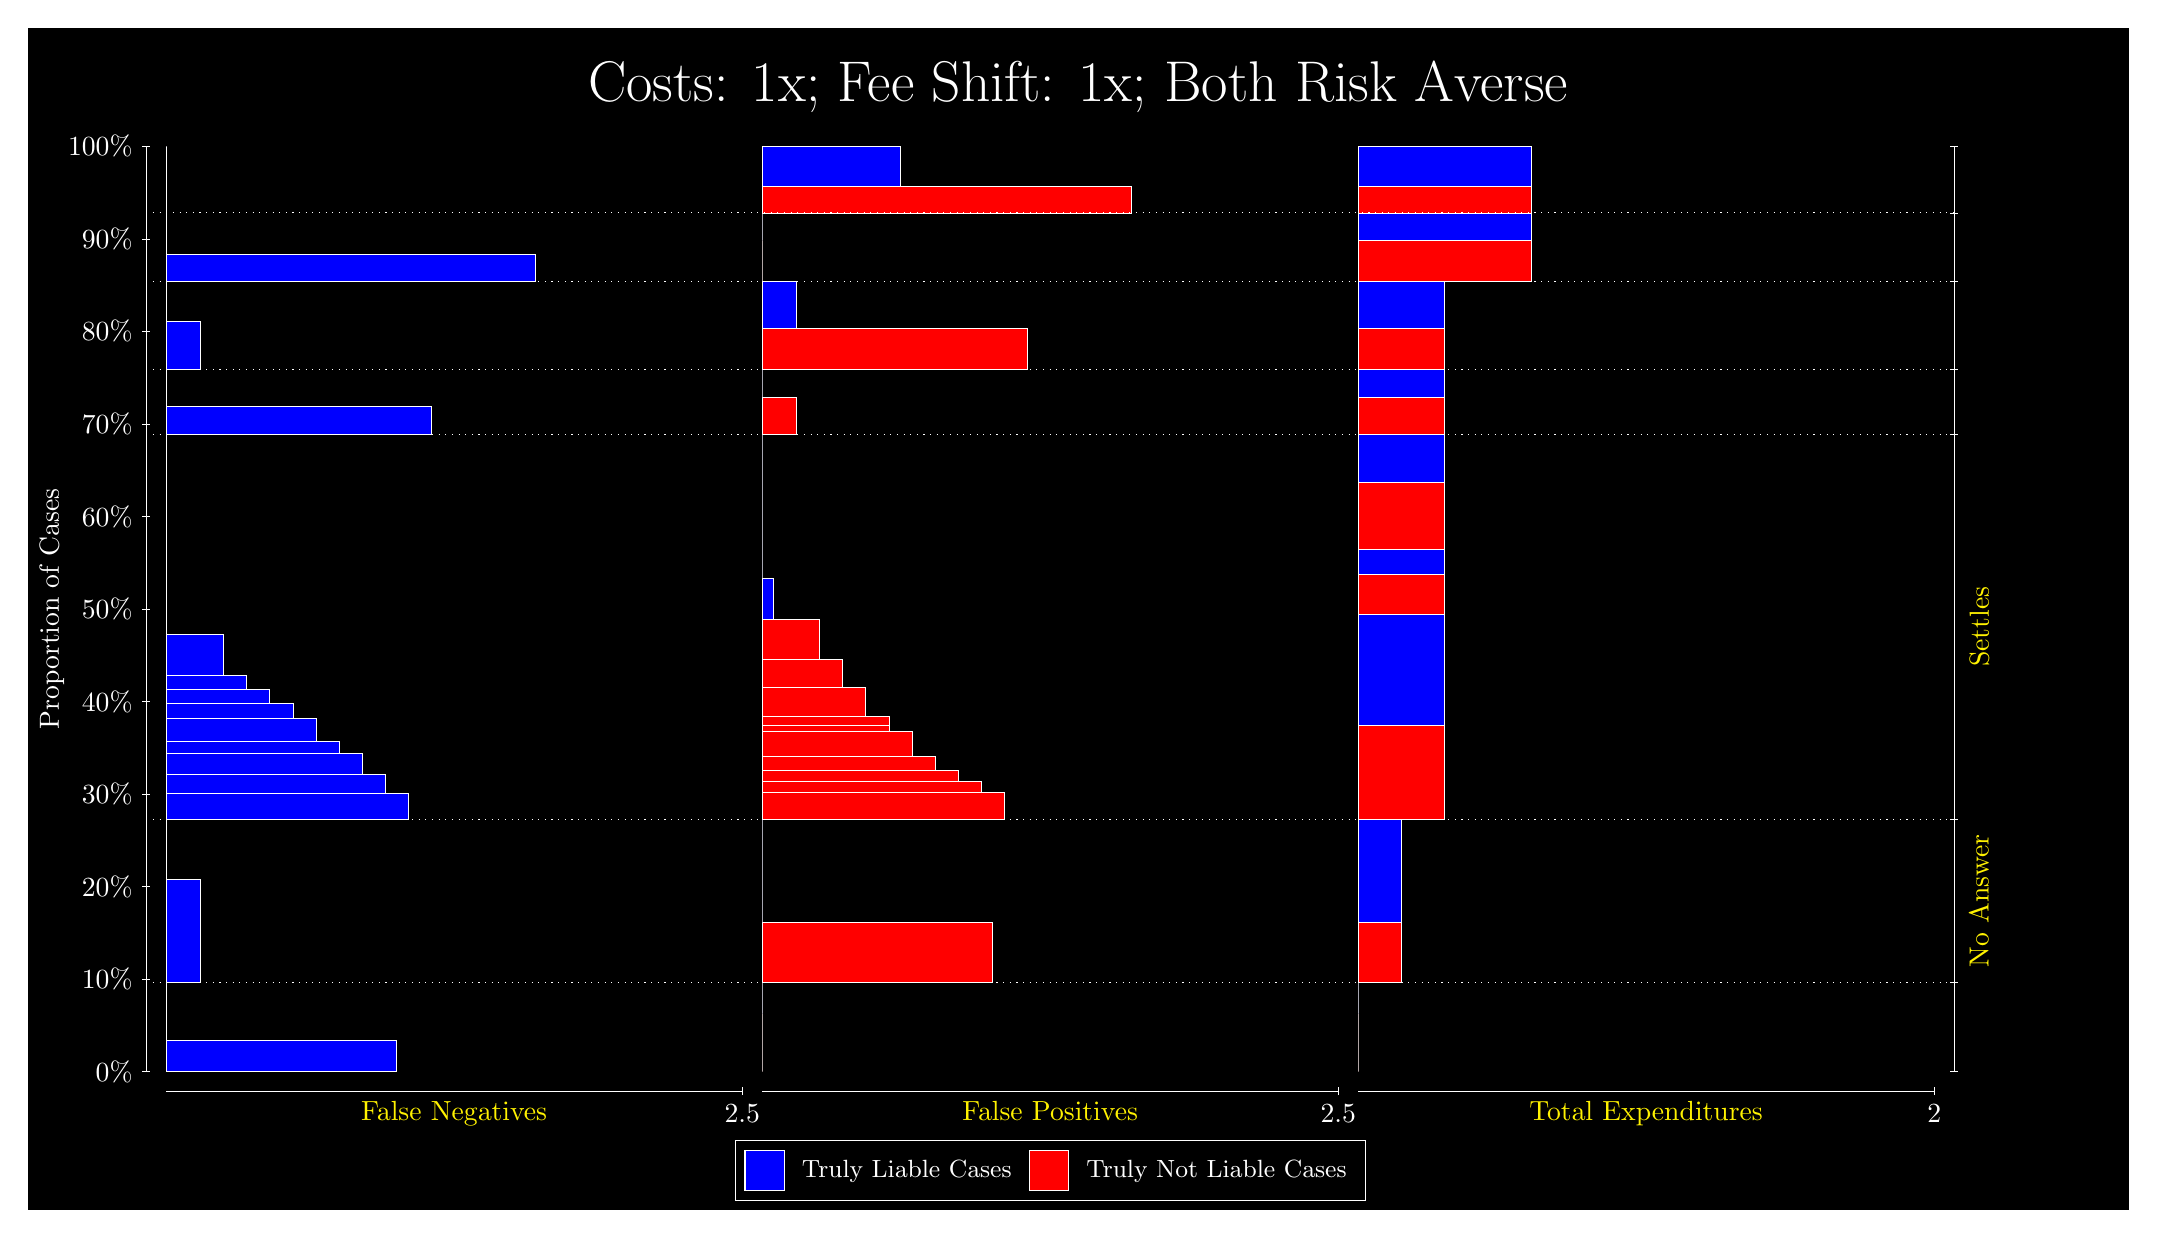
\begin{tikzpicture}
\draw[fill=black] (0,0) rectangle (26.667,15);
\draw[text=white] (0,13.5) rectangle (26.667,15) node[midway] {\huge Costs: 1x; Fee Shift: 1x; Both Risk Averse};
\draw[white, very thin] (1.5,1.75) -- (1.5,13.5);
\node[rotate=90, text=white, anchor=center] at (0.3, 7.625) {Proportion of Cases};
\draw[white, very thin] (1.45,1.75) -- (1.55,1.75);
\node[text=white, anchor=east] at (1.45, 1.75) {0\%};
\draw[white, very thin] (1.45,2.925) -- (1.55,2.925);
\node[text=white, anchor=east] at (1.45, 2.925) {10\%};
\draw[white, very thin] (1.45,4.1) -- (1.55,4.1);
\node[text=white, anchor=east] at (1.45, 4.1) {20\%};
\draw[white, very thin] (1.45,5.275) -- (1.55,5.275);
\node[text=white, anchor=east] at (1.45, 5.275) {30\%};
\draw[white, very thin] (1.45,6.45) -- (1.55,6.45);
\node[text=white, anchor=east] at (1.45, 6.45) {40\%};
\draw[white, very thin] (1.45,7.625) -- (1.55,7.625);
\node[text=white, anchor=east] at (1.45, 7.625) {50\%};
\draw[white, very thin] (1.45,8.8) -- (1.55,8.8);
\node[text=white, anchor=east] at (1.45, 8.8) {60\%};
\draw[white, very thin] (1.45,9.975) -- (1.55,9.975);
\node[text=white, anchor=east] at (1.45, 9.975) {70\%};
\draw[white, very thin] (1.45,11.15) -- (1.55,11.15);
\node[text=white, anchor=east] at (1.45, 11.15) {80\%};
\draw[white, very thin] (1.45,12.325) -- (1.55,12.325);
\node[text=white, anchor=east] at (1.45, 12.325) {90\%};
\draw[white, very thin] (1.45,13.5) -- (1.55,13.5);
\node[text=white, anchor=east] at (1.45, 13.5) {100\%};

\draw[white, very thin] (24.457,1.75) -- (24.457,13.5);
\draw[white, very thin] (24.407,1.75) -- (24.507,1.75);
\node[anchor=west] at (24.407, 1.75) {};
\draw[white, very thin] (24.407,2.8861) -- (24.507,2.8861);
\node[anchor=west] at (24.407, 2.8861) {};
\draw[white, very thin] (24.407,4.9507) -- (24.507,4.9507);
\node[anchor=west] at (24.407, 4.9507) {};
\draw[white, very thin] (24.407,9.8451) -- (24.507,9.8451);
\node[anchor=west] at (24.407, 9.8451) {};
\draw[white, very thin] (24.407,10.669) -- (24.507,10.669);
\node[anchor=west] at (24.407, 10.669) {};
\draw[white, very thin] (24.407,11.785) -- (24.507,11.785);
\node[anchor=west] at (24.407, 11.785) {};
\draw[white, very thin] (24.407,12.656) -- (24.507,12.656);
\node[anchor=west] at (24.407, 12.656) {};
\draw[white, very thin] (24.407,13.5) -- (24.507,13.5);
\node[anchor=west] at (24.407, 13.5) {};

\draw[white, very thin, fill=blue] (1.75,1.75) rectangle (4.6775,2.1504);
\draw[white, very thin, fill=red] (1.75,2.1504) rectangle (1.75,2.8861);
\draw[white, very thin, fill=blue] (1.75,2.8861) rectangle (2.1891,4.1973);
\draw[white, very thin, fill=red] (1.75,4.1973) rectangle (1.75,4.9507);
\draw[white, very thin, fill=blue] (1.75,4.9507) rectangle (4.8239,5.2787);
\draw[white, very thin, fill=blue] (1.75,5.2787) rectangle (4.5312,5.5203);
\draw[white, very thin, fill=blue] (1.75,5.5203) rectangle (4.2384,5.7871);
\draw[white, very thin, fill=blue] (1.75,5.7871) rectangle (3.9457,5.9505);
\draw[white, very thin, fill=blue] (1.75,5.9505) rectangle (3.6529,6.2416);
\draw[white, very thin, fill=blue] (1.75,6.2416) rectangle (3.3602,6.4252);
\draw[white, very thin, fill=blue] (1.75,6.4252) rectangle (3.0674,6.5991);
\draw[white, very thin, fill=blue] (1.75,6.5991) rectangle (2.7746,6.7783);
\draw[white, very thin, fill=blue] (1.75,6.7783) rectangle (2.4819,7.3014);
\draw[white, very thin, fill=red] (1.75,7.3014) rectangle (1.75,9.8451);
\draw[white, very thin, fill=blue] (1.75,9.8451) rectangle (5.1167,10.203);
\draw[white, very thin, fill=red] (1.75,10.203) rectangle (1.75,10.669);
\draw[white, very thin, fill=blue] (1.75,10.669) rectangle (2.1891,11.272);
\draw[white, very thin, fill=red] (1.75,11.272) rectangle (1.75,11.785);
\draw[white, very thin, fill=blue] (1.75,11.785) rectangle (6.4341,12.135);
\draw[white, very thin, fill=red] (1.75,12.135) rectangle (1.75,12.656);
\draw[white, very thin, fill=red] (1.75,12.656) rectangle (1.75,12.998);
\draw[white, very thin, fill=blue] (1.75,12.998) rectangle (1.75,13.5);
\draw[white, very thin, fill=red] (9.3189,1.75) rectangle (9.3189,2.4857);
\draw[white, very thin, fill=blue] (9.3189,2.4857) rectangle (9.3189,2.8861);
\draw[white, very thin, fill=red] (9.3189,2.8861) rectangle (12.246,3.6394);
\draw[white, very thin, fill=blue] (9.3189,3.6394) rectangle (9.3189,4.9507);
\draw[white, very thin, fill=red] (9.3189,4.9507) rectangle (12.393,5.2984);
\draw[white, very thin, fill=red] (9.3189,5.2984) rectangle (12.1,5.432);
\draw[white, very thin, fill=red] (9.3189,5.432) rectangle (11.807,5.5716);
\draw[white, very thin, fill=red] (9.3189,5.5716) rectangle (11.515,5.7588);
\draw[white, very thin, fill=red] (9.3189,5.7588) rectangle (11.222,6.0696);
\draw[white, very thin, fill=red] (9.3189,6.0696) rectangle (10.929,6.1433);
\draw[white, very thin, fill=red] (9.3189,6.1433) rectangle (10.929,6.2568);
\draw[white, very thin, fill=red] (9.3189,6.2568) rectangle (10.636,6.6334);
\draw[white, very thin, fill=red] (9.3189,6.6334) rectangle (10.344,6.9888);
\draw[white, very thin, fill=red] (9.3189,6.9888) rectangle (10.051,7.4944);
\draw[white, very thin, fill=blue] (9.3189,7.4944) rectangle (9.4652,8.0175);
\draw[white, very thin, fill=blue] (9.3189,8.0175) rectangle (9.3189,9.8451);
\draw[white, very thin, fill=red] (9.3189,9.8451) rectangle (9.758,10.311);
\draw[white, very thin, fill=blue] (9.3189,10.311) rectangle (9.3189,10.669);
\draw[white, very thin, fill=red] (9.3189,10.669) rectangle (12.686,11.183);
\draw[white, very thin, fill=blue] (9.3189,11.183) rectangle (9.758,11.785);
\draw[white, very thin, fill=red] (9.3189,11.785) rectangle (9.3189,12.305);
\draw[white, very thin, fill=blue] (9.3189,12.305) rectangle (9.3189,12.656);
\draw[white, very thin, fill=red] (9.3189,12.656) rectangle (14.003,12.998);
\draw[white, very thin, fill=blue] (9.3189,12.998) rectangle (11.075,13.5);
\draw[white, very thin, fill=red] (16.888,1.75) rectangle (16.888,2.4857);
\draw[white, very thin, fill=blue] (16.888,2.4857) rectangle (16.888,2.8861);
\draw[white, very thin, fill=red] (16.888,2.8861) rectangle (17.437,3.6394);
\draw[white, very thin, fill=blue] (16.888,3.6394) rectangle (17.437,4.9507);
\draw[white, very thin, fill=red] (16.888,4.9507) rectangle (17.986,6.1433);
\draw[white, very thin, fill=blue] (16.888,6.1433) rectangle (17.986,7.5546);
\draw[white, very thin, fill=red] (16.888,7.5546) rectangle (17.986,8.0602);
\draw[white, very thin, fill=blue] (16.888,8.0602) rectangle (17.986,8.3882);
\draw[white, very thin, fill=red] (16.888,8.3882) rectangle (17.986,9.2338);
\draw[white, very thin, fill=blue] (16.888,9.2338) rectangle (17.986,9.8451);
\draw[white, very thin, fill=red] (16.888,9.8451) rectangle (17.986,10.311);
\draw[white, very thin, fill=blue] (16.888,10.311) rectangle (17.986,10.669);
\draw[white, very thin, fill=red] (16.888,10.669) rectangle (17.986,11.183);
\draw[white, very thin, fill=blue] (16.888,11.183) rectangle (17.986,11.785);
\draw[white, very thin, fill=red] (16.888,11.785) rectangle (19.083,12.305);
\draw[white, very thin, fill=blue] (16.888,12.305) rectangle (19.083,12.656);
\draw[white, very thin, fill=red] (16.888,12.656) rectangle (19.083,12.998);
\draw[white, very thin, fill=blue] (16.888,12.998) rectangle (19.083,13.5);
\draw[white, dotted] (1.5,2.8861) -- (24.457,2.8861);
\draw[white, dotted] (1.5,4.9507) -- (24.457,4.9507);
\draw[white, dotted] (1.5,9.8451) -- (24.457,9.8451);
\draw[white, dotted] (1.5,10.669) -- (24.457,10.669);
\draw[white, dotted] (1.5,11.785) -- (24.457,11.785);
\draw[white, dotted] (1.5,12.656) -- (24.457,12.656);
\draw[white, very thin] (1.75,1.5) -- (9.0689,1.5);
\node[text=yellow, anchor=north] at (5.4094, 1.5) {False Negatives};
\draw[white, very thin] (9.0689,1.45) -- (9.0689,1.55);
\node[text=white, anchor=north] at (9.0689, 1.45) {2.5};

\draw[white, very thin] (9.3189,1.5) -- (16.638,1.5);
\node[text=yellow, anchor=north] at (12.978, 1.5) {False Positives};
\draw[white, very thin] (16.638,1.45) -- (16.638,1.55);
\node[text=white, anchor=north] at (16.638, 1.45) {2.5};

\draw[white, very thin] (16.888,1.5) -- (24.207,1.5);
\node[text=yellow, anchor=north] at (20.547, 1.5) {Total Expenditures};
\draw[white, very thin] (24.207,1.45) -- (24.207,1.55);
\node[text=white, anchor=north] at (24.207, 1.45) {2};


\node[text=yellow, centered, rotate=90] at (24.777, 3.9184) {No Answer};
\node[text=yellow, centered, rotate=90] at (24.777, 7.3979) {Settles};





\draw (12.978300999999998,1.5) node[draw=none] (baseCoordinate) {};
\begin{scope}[align=center]
        \matrix[scale=0.5, draw=white, below=0.5cm of baseCoordinate, nodes={draw}, column sep=0.1cm]{
            \node[rectangle, draw, minimum width=0.5cm, minimum height=0.5cm, fill=blue] {}; &
            \node[draw=none, font=\small, text=white] (B) {Truly Liable Cases}; &
            \node[rectangle, draw, minimum width=0.5cm, minimum height=0.5cm, fill=red] {}; &
            \node[draw=none, font=\small, text=white] (B) {Truly Not Liable Cases}; \\
            };
\end{scope}

\end{tikzpicture}
\end{document}